%_______________________________________________________________________________
%class
%_______________________________________________________________________________
%\documentclass[a4paper,11pt,onecolumn,final,german,openbib]{scrbook}
\documentclass[a4paper,11pt,oneside,final,english,toc=bib,draft]{scrbook}

% fonts

\usepackage{fontspec}
\setmainfont{Libre Baskerville} % Libre Baskerville - Palatino Linotype - Constantia
\setsansfont{Helvetica} % Arial
\setmonofont{Consolas} % Hack

\usepackage[OT1]{eulervm}
% \usepackage{mathdesign}

%_______________________________________________________________________________
% page borders
%_______________________________________________________________________________
\addtolength{\headheight}{2cm}
%\addtolength{\topmargin}{2cm}
\setlength{\oddsidemargin}{1.0cm}
\setlength{\evensidemargin}{0.5cm}
\setlength{\textwidth}{14.3cm}
\setlength{\parindent}{0mm}

%_______________________________________________________________________________
% packages
%_______________________________________________________________________________
% \usepackage{german}
\usepackage{babel}[uk-english]
% \usepackage{textcomp}
\usepackage{csquotes}

\usepackage{mathtools}
\usepackage{amssymb,amsfonts}
% \usepackage{physics}
\usepackage[separate-uncertainty=true,per-mode=power,group-separator={,}]{siunitx} % ,per-mode=fraction 
% \usepackage[version=4]{mhchem}
% \usepackage{dsfont}
% \usepackage{slashed}

\usepackage{graphicx}
\usepackage{xcolor}
% \usepackage{subfigure}
\usepackage{float}
\usepackage{caption}
\usepackage{subcaption}
\usepackage{enumitem}

% \usepackage{url}
% \usepackage{enumerate}

\usepackage{booktabs}
% \usepackage{multirow}

% \usepackage{appendix}

\usepackage{todonotes}

\usepackage[style=ieee]{biblatex} % ,sorting=none style=h-physrev3 defernumbers=true
\bibliography{thesis}


\graphicspath{ {./images/} }

\usepackage[draft=false]{hyperref}
\hypersetup{
  colorlinks=true,
  linkcolor=blue,
  citecolor=teal
}

\captionsetup[figure]{labelfont=bf,format=plain,labelsep=newline} % ,labelsep=period ,margin=1cm
\captionsetup[table]{labelfont=bf,format=hang,labelsep=space} % ,labelsep=period ,margin=1cm ,labelsep=newline

\renewcommand{\arraystretch}{1.2}

\newcommand{\figwidth}{12cm}

\parindent10mm

% \makesavenoteenv{table}

\usepackage{mgscience}

%_______________________________________________________________________________
% bold fonts for headings
%_______________________________________________________________________________
\font\afont=cmssbx10 scaled \magstep5     % for the title
\font\bfont=cmssbx10 scaled \magstep4     % for chapter headings
\font\cfont=cmssbx10 scaled \magstep3
\font\dfont=cmssbx10 scaled \magstep2     % for section headings and author name
\font\efont=cmssbx10 scaled \magstephalf

%_______________________________________________________________________________
% index depth
%_______________________________________________________________________________
\setcounter{secnumdepth}{3}
\setcounter{tocdepth}{3}

%_______________________________________________________________________________
% new commands
%_______________________________________________________________________________
% \newcommand{\demi}{\frac{1}{2}}

%_______________________________________________________________________________
% renewed commands
%_______________________________________________________________________________
% \renewcommand{\topfraction}{1.}       % this is important for figure placement
% \renewcommand{\bottomfraction}{1.}
\makeatletter
\renewcommand\paragraph{\@startsection{paragraph}{4}{\z@}%
  {-3.25ex\@plus -1ex \@minus -.2ex}%
  {1.5ex \@plus .2ex}%
  {\normalfont\normalsize\bfseries}
}
\makeatother

%_______________________________________________________________________________
% special words, hyphenation
%_______________________________________________________________________________
% \hyphenation{Ba-che-lor-ar-beit}

\pagestyle{empty}
\pagestyle{headings}
%for changing the style on a specific page use \thispagestyle{e.g., empty}

%_______________________________________________________________________________
%_______________________________________________________________________________
\begin{document}
\pagenumbering{roman}

%_______________________________________________________________________________
\begin{titlepage}
  \vspace*{6mm}
  \begin{center}
     {\afont Comparison of 3-dimensional chromatin structures based on single cell Hi-C data}
     \\[3.5cm]
     {\large von}
     \\[3.5cm]
     {\dfont Moritz Gmeiner}
     \\[1.5cm]
     {\dfont Supervisor: PD Dr. Peter Virnau}
     \\[2cm]
     % {\large Bachelorarbeit in Physik \/\\
     %    vorgelegt dem Fachbereich Physik, Mathematik und Informatik (FB 08) \/\\
     %    der Johannes Gutenberg-Universität Mainz \/\\
     %    am 1. April 2012}
     {\large Bachelor Thesis in Physics \/\\
        presented to the faculty physics, mathematics, and computer science (FB 08) \/\\
        of the Johannes Gutenberg University Mainz \/\\
        \today}
   \end{center}
   \vfill
   1. Reviewer: PD Dr. Peter Virnau \\	
   2. Reviewer: Prof. Dr. Friederike Schmid \\
   \vfill
\end{titlepage}

\thispagestyle{empty}
Ich versichere, dass ich die Arbeit selbstständig verfasst und keine 
anderen als die angegebenen Quellen und Hilfsmittel benutzt sowie 
Zitate kenntlich gemacht habe.
\\
\\[3.5cm] 
Mainz, den \today
\vfill
\noindent 
Moritz Gmeiner\\
KOMET\\
Institut für Physik\\
Staudingerweg 7\\
Johannes Gutenberg-Universität
D-55099 Mainz\\
{ \texttt{mgmeiner@students.uni-mainz.de} }

%_______________________________________________________________________________
% \renewcommand\contentsname{Inhaltsverzeichnis}
% \renewcommand\figurename{Abbildung}
% \renewcommand\tablename{Tabelle}

\tableofcontents
\clearpage

\mainmatter
\sloppy

%_______________________________________________________________________________
% \include{...}
\chapter{Introduction} % (fold)
\label{cha:introduction}

{\em Dieses Dokument richtet sich an Studierende am Fachbereich 08 im 
Studiengang Bachelor of Science (Physik). Sie finden hier Beispiele 
für eine mögliche Gliederung Ihrer Arbeit und Hinweise zur 
Strukturierung des Inhalts. Selbstverständlich sollen Sie diese 
Gliederung nach den Gegebenheiten Ihrer Bachelorarbeit anpassen. 
Besprechen Sie rechtzeitig mit Ihrem Betreuer, ob Ihr Entwurf sinnvoll 
ist. Holen Sie sich auch Anregungen zur Gestaltung von Abschlussarbeiten 
aus der Literatur (siehe z.\ B.\ \verb|\cite{EbelBliefert}|).}

\medskip

\textcolor{orange}{In der Einleitung Ihrer Bachelorarbeit sollte das Thema der Arbeit 
möglichst allgemeinverständlich eingeführt werden. Gehen Sie 
dabei auch auf das weitere Umfeld der Arbeit ein und erläutern Sie, 
warum Aufgabenstellung und Herangehensweise interessant sind. Auch 
die weitere Gliederung kann angesprochen werden, um dem Leser einen 
ersten überblick über den nachfolgenden Text zu geben.}

\bigskip

The goal of this thesis is to explore the chromatin structure of DNA in the nucleus further, based mainly on previous the research in \cite{wettermann_minimal_2020}.

DNA is in the nucleus. Structure of DNA is important. DNA structure is lost during mitosis and has to reestablished later. Structure is important for transcription and differentiation.

\bigskip



%_______________________________________________________________________________
% \chapter{Main Part}

% Die typische Gliederung einer Bachelorarbeit könnte so aussehen, 
% wie im folgenden dargestellt. 
% \medskip

% Verwenden Sie aussagekräftige Kapitelüberschriften, also zum 
% Beispiel {\em Aufbau eines Teilchenbeschleunigers} statt 
% {\em Versuchsaufbau}.


% chapter introduction (end)

%_______________________________________________________________________________
\chapter{Simulation} % (fold)
\label{cha:simulation}

\section{Model and Simulation Protocol} % (fold)
\label{sec:model_and_simulation_protocol}

The simulation protocol was for the most part carried over from \cite{wettermann_minimal_2020}. The main file for simulating the genome structure of an entire cell is \verb|simulate_cell.py|. Additionally simulations of single chromosomes were carried out; the protocol for these simulations is identical to those of the entire genome, except only the chromosome in question was modelled . The simulation is a molecular dynamics simulation using the HOOMD-blue\cite{anderson_hoomd-blue_2020} toolkit. Each chromosome is modelled as beads on a string, where each bead represents a bin of \(\SI{100000}{bp}\). This is the same resolution as was chosen in \cite{wettermann_minimal_2020}, and represents a compromise between the resolution of our simulation and the \textcolor{orange}{resolution}\todo{find better word} of the contact data we have available: a higher resolution, i.e. a smaller bin size of for example \(\SI{40000}{bp}\), would increase the resolution of our simulation and enable us to see smaller structures, but at the same time would spread our fixed number of contacts across a higher number of beads. This would make in particular make the effect of having captured only a fraction of all possible contacts more prominent. \todo{insert reference to table of fraction of contacts captured}. Vice versa, decreasing the bin size would help mitigate the partial capture of contacts, but limit our spatial resolution in the simulation. With this resolution our genome is represented by 20 chains varying in length between 500 and 2,000 beads (the exact lengths for each chromosome can be found in Table~\ref{tab:chrom_lengths}), or 25,714 beads in total. This does not represent the entirety of the mouse genome, whose length is approximately \(\SI{2632}{Mbp}\)\footnote{Mouse Genome Assembly GRCm39 from \url{https://www.ncbi.nlm.nih.gov/grc/mouse/data}, visited on 26.02.2022}, or 26,321 beads at our resolution of \(\SI{100000}{bp \per bead}\). The reason for this is that all beads at the boundary of a chromosome, that had no contact in any of the eight cells, were dropped from the simulation, since their impact was assumed to be only very marginal. Boundary beads that had contacts in some cells but not others were kept in the simulation of all cell in order to keep the simulation data comparable across cells.

The model itself is a generic bead-spring polymer model in which three kinds of bonds are defined. The first two kind of bonds are harmonic bonds between two beads with the general protential

\[
  V(r) = \frac{2} \kappa \left( r - r_0 \right)^2
\]

where \(\kappa\) is the force constant determining the stiffness of the bond and \(r_0\) is the preferred bond distance. The first kind of harmonic bonds are the backbone bonds connecting adjacent beads in each chromosome. For these bonds \(\kappa = 2000\) and \(r_0 = 1.0 \). The other harmonic bonds in the simulation are the pre-defined contacts derived from the Hi-C data set from\cite{stevens_3d_2017}. Here, again a force constant of \(\kappa = 2000\) is chosen, the preferred bond distance on the other hand is set a little bit larger at \(r_0 = 1.5\) in accordance with \cite{wettermann_minimal_2020}. The third kind of bond is a Gaussian pair potential of the form

\[
  V(r) = \begin{cases}
    \epsilon \exp \left[ - \frac{2} \left( \frac{r}{\sigma} \right)^2 \right] & r < r_\text{cut} \\
    0 & r \geq r_\text{cut}
  \end{cases}
\]

between all beads designed to push all non-bonded beads away from each other. This potential is used in 2 forms in different steps of the simulation: a full form with \(\sigma = 1.0\) and \(r_\text{cut} = 3.5\) and a reduced form with \(\sigma = 0.1\) and \(r_\text{cut} = 0.4\). In both cases \(\epsilon = 100\). On one hand, this reproduced the fact that at physiological conditions DNA is negatively charged and thus repels each other. \textcolor{orange}{On the other hand it represents an excluded volume potential that pushes all beads away from each other}\todo{Rewrite?}. An overview of all the potentials in the simulation can be seen in Figure~\ref{img:potentials}.

\begin{figure}[ht]
\centering
  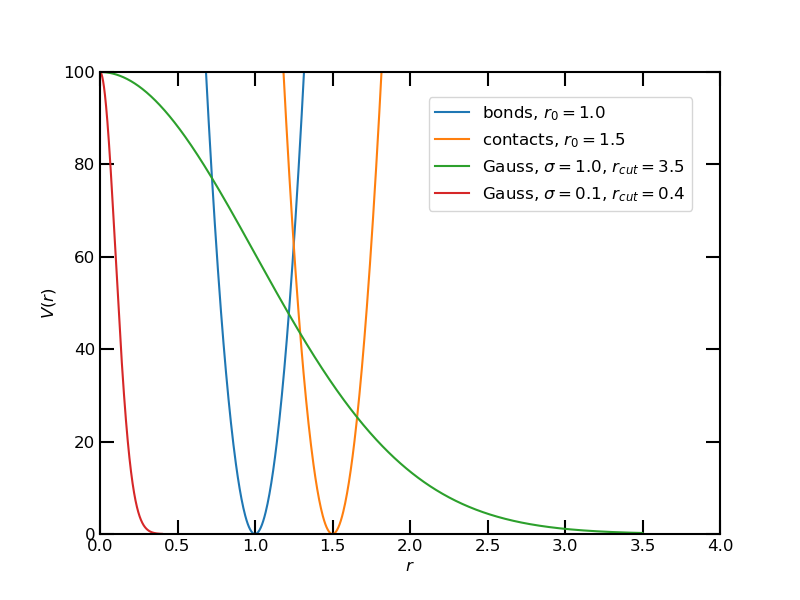
\includegraphics[width=\figwidth]{potentials.png}
  \caption{Potentials used in the simulation. Bonds and contacts are harmonic potentials of the form \(V(r) = 1000 (r - r_0)^2\), with bonds having an \(r_0\) of 1.0 and contacts gaving an \(r_0\) of 1.5. Gauss potentials are of the form \(V(r) = 100 \exp\left[- \frac{2} \left( \frac{r}{\sigma} \right)^2 \right]\) and are set to 0 for \(r\) greater than the cutoff value \(r_\text{cut}\).}
  \label{img:potentials}
\end{figure}

The system is initalised by distributing all the beads randomly throughout the simulation box (uniform distribution, using \verb|numpy.uniform.random|\cite{harris_array_2020}). The bonds are set and the simulation is repeatedly run using a Langevin integrator (\verb|hoomd.md.integrate.langevin|\cite{anderson_hoomd-blue_2020}, \(dt=0.001\), \(kT = 1.0\)) through the following steps:

\begin{itemize}[label=\(\bullet\)]
  \item 80,000 time steps with no excluded volume potentials
  \item 50,000 time steps with reduced volume potentials
  \item 50,000 time steps with full excluded volume potentials
\end{itemize}

Bonds and contacts are active at all of those steps. After each cycle the current state is saved to a \verb|.gsd| trajectory file. These steps were repeated in each simulation for a total of 105 cycles. The first few cycles have to be discarded as the system takes some time to find its ground state, although certain problems can arise here that will be discussed later in \ref{sec:problems_with_the_simulation}.

% section model_and_simulation_protocol (end)

\section{Simulation results} % (fold)
\label{sec:simulation_results}

Each simulation will yield 105 sequential configuration, i.e. the simulation state is not reset after each simulation cycle , but instead the final state of each cycle is the initial state of the next cycle. This has the advantage of giving the system time to \textcolor{orange}{tune in}\todo{better word? \enquote{einschwingen}}, but also the disadvantage of the possiblility that certain end configurations will never be reached in a simulation run after it has tuned in to a different locally minimal configuration. The potential energies of the simulation run of cell 2 can be seen in Figure~\ref{img:potential_energy_cell2}. While the first two configurations show a potential energy significantly larger than the later ones, the system quickly converges to a potential energy of about \(\num{7950000}\) and then shows only small deviations of less than \(1 \%\). Thus both the length of the settling period and the potential energy of the configurations matches \cite{wettermann_minimal_2020} extremely well. \textcolor{orange}{To minimise the effect of the settling period the first 5 configurations of each simulation run will generally be excluded in all subsequent analyses where the data from all configurations are combined.}

Likewise, Figure~\ref{img:distance_pdf_cell2} shows the distance distribution of the bonds and (predetermined) contacts across all configurations of the simulation of cell 2. The results are again very similar to \cite{wettermann_minimal_2020}, with both peaks and means shifted slightly to the right. The \(99.73\)th quartile is at \(1.713\) for bonds and \(2.418\) for contacts, showing that most bonds and contacts are enforced reasonably well.

\begin{figure}[ht]
\centering
  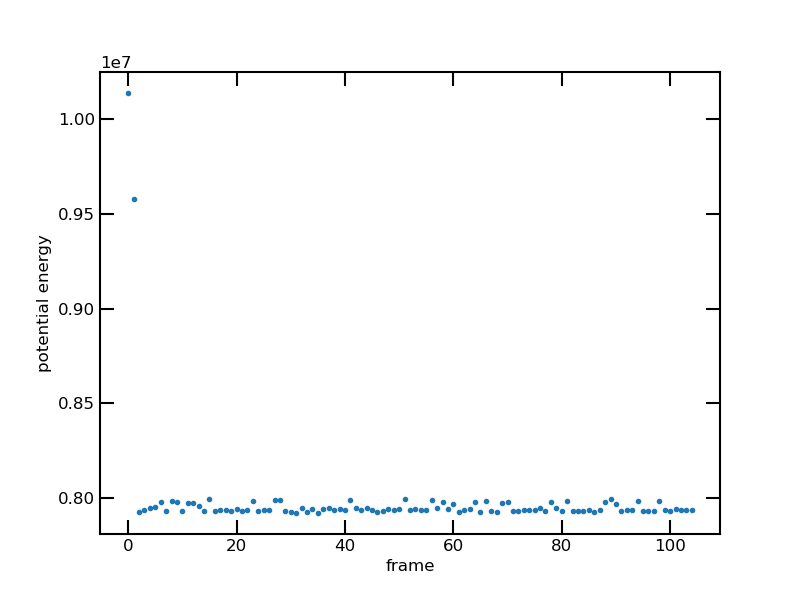
\includegraphics[width=12cm]{potential_energy_cell2.png}
  \caption{\textcolor{red}{CAPTION}}
  \label{img:potential_energy_cell2}
\end{figure}

\begin{figure}[ht]
\centering
  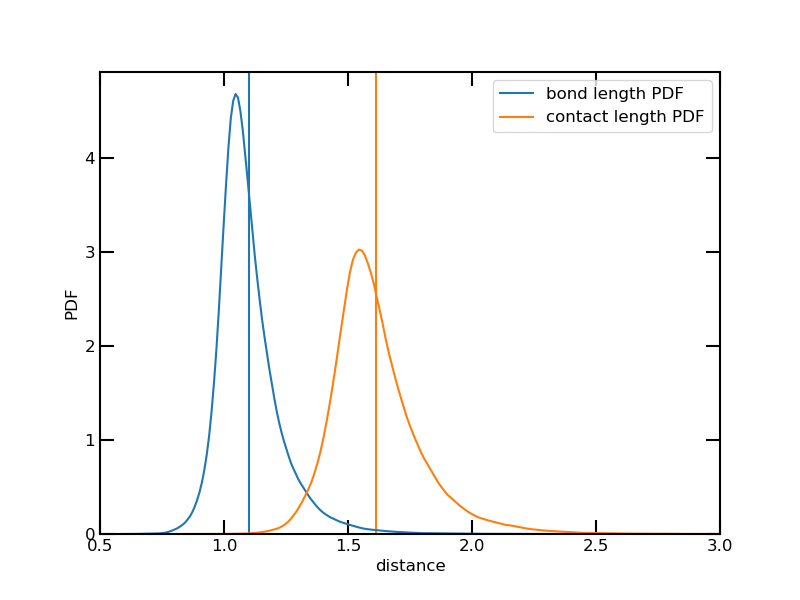
\includegraphics[width=12cm]{distance_pdf_cell2.png}
  \caption{\textcolor{red}{CAPTION} bond mean: \(\num{1.099}\) ; bonds \(99.73\%\) percentile: \(1.713\) ; contacts mean: \(\num{1.613}\) ; contact \(99.73\%\) percentile: \(2.418\)}
  \label{img:distance_pdf_cell2}
\end{figure}

For the other cells the situation is generally similar, except for cell 1 and cell 5, which will be dicussed separately in \ref{sec:problems_with_the_simulation}. The standard deviations of potential energies are between \(0.3\%\) and \(1.8\%\) of the mean, showing the minimum energy configuration to be quite stable in these cells. Also neither bonds nor contacts are overly overstretched in any cells, including cell 1 and cell 5. A complete overview of potential energy percentage standard deviations and mean and \(99.73\)th percentile for bonds and contacts can be found in Table~\ref{tab:simulation_pe_dists}.

% section simulation_results (end)

\section{Problems with the simulation} % (fold)
\label{sec:problems_with_the_simulation}

% section problems_with_the_simulation (end)


% chapter simulation (end)

\chapter{Comparison of Cells} % (fold)
\label{cha:comparison_of_cells}

% chapter comparison_of_cells (end)

\chapter{Individual Chromosomes} % (fold)
\label{cha:individual_chromosomes}

% chapter individual_chromosomes (end)

%_______________________________________________________________________________
\chapter{Conclusion} % (fold)
\label{cha:conclusion}

In der Zusammenfassung sollten Sie in knapper Form die Aufgabenstellung 
und die wichtigsten Ergebnisse rekapitulieren. Es ist für die 
Gutachter hilfreich, wenn Sie ausdrücklich beschreiben, worin 
Ihre eigenen Beiträge liegen. Scheuen Sie sich auch nicht davor 
auszusprechen, welche Untersuchungen durch die Zeitbegrenzung der 
Bachelorarbeit nicht möglich waren und nutzen Sie dies als 
überleitung zu einem Ausblick auf mögliche weitergehende 
Arbeiten an der Aufgabenstellung.

% chapter conclusion (end)

%_______________________________________________________________________________
\appendix

% \chapter{Appendix}
\chapter{Tables and Figures} % (fold)
\label{cha:tables_and_figures}

\textcolor{orange}{In der Regel sind die in Tabellen und Abbildungen enthalten Informationen 
so wichtig, dass sie im Hauptteil der Arbeit erscheinen sollten. Unter 
Umständen sind aber ergänzende Tabellen und Abbildungen gut in einem 
Anhang aufgehoben. Wie im Hauptteil sollten Sie auch hier darauf achten, 
dass die in Tabellen und Figuren (siehe Abb.\ ref{Abb:1}) dargestellte 
Information im Text angesprochen wird und selbsterklärende Legenden}
vorhanden sind.

\medskip

\begin{table}[H]
\centering
  \caption{\textcolor{red}{MAKE CAPTION}}
  \label{tab:chrom_lengths}
  \begin{tabular}{c c c c c c c c c c c}
   \toprule
    Chrom & 1 & 2 & 3 & 4 & 5 & 6 & 7 & 8 & 9 & 10 \\
    Length & 1924 & 1791 & 1570 & 1534 & 1488 & 1466 & 1424 & 1263 & 1215 & 1275 \\
  \midrule
    Chrom & 11 & 12 & 13 & 14 & 15 & 16 & 17 & 18 & 19 & X \\
    Length & 1189 & 1171 & 1174 & 1218 & 1010 & 952 & 919 & 876 & 584 & 1671 \\
  \bottomrule
  \end{tabular}
\end{table}

\begin{table}[ht]
\centering
  \caption{\textcolor{red}{MAKE CAPTION}}
  \label{tab:simulation_pe_dists}
  \begin{tabular}{S @{\phantom{abc}} S @{\phantom{abc}} S @{\phantom{abc}} S @{\phantom{abc}} S @{\phantom{abc}} S}
  \toprule
    {Cell} & {PE \% deviation} & \multicolumn{2}{c}{bonds} & \multicolumn{2}{c}{contacts} \\
     & & {mean} & {99.73th prct} & {mean} & {99.73th prct} \\
  \midrule
    1 & 8.51\% & 1.13 & 1.98 & 1.62 & 2.72 \\
    2 & 0.27\% & 1.10 & 1.71 & 1.61 & 2.42 \\
    3 & 0.67\% & 1.14 & 1.88 & 1.68 & 2.52 \\
    4 & 1.83\% & 1.14 & 2.08 & 1.61 & 2.46 \\
    5 & 8.63\% & 1.11 & 1.81 & 1.62 & 2.55 \\
    6 & 0.94\% & 1.16 & 2.07 & 1.61 & 2.38 \\
    7 & 0.29\% & 1.10 & 1.58 & 1.59 & 2.09 \\
    8 & 0.28\% & 1.08 & 1.56 & 1.60 & 2.25 \\
  \bottomrule
  \end{tabular}
\end{table}

% chapter tables_and_figures (end)

\chapter{Used software} % (fold)
\label{cha:used_software}

\begin{table}[H]
\centering
\label{tab:used_software}
\caption{Software used for simulation and data analysis. Two systems were used, the top one a Manjaro Linux (based on Arch Linux) system and the bottom one a Microsoft Windows system with Anaconda}
  \begin{tabular}{c @{\phantom{abc}} c @{\phantom{abc}} c}
  \toprule
    Package & Version & Package Source \\
  \midrule
    HOOMD-blue & 1.9.7 & built from source \\
    numpy &  & arch repo \\
    scipy &  & arch repo \\
    pandas &  & arch repo \\
    matplotlib &  & arch repo \\
    gsd & & \\
    vmd & & \\
  \midrule
    numpy & 1.20.3 & anaconda \\
    scipy & 1.7.1 & anaconda \\
    pandas & 1.3.4 & anaconda \\
    matplotlib & 3.4.3 & anaconda \\
    gsd & 2.5.1 & pip \\
    hicreppy & 771cf72 & github \\
  \bottomrule
  \end{tabular}
\end{table}

\todo{packages and versions for linux system}


% chapter used_software (end)

%_______________________________________________________________________________
\chapter{Weiterführende Details zur Arbeit} % (fold)
\label{cha:weiterführende_details_zur_arbeit}

Manch wichtiger Teil Ihrer tatsächlichen Arbeit ist zu technisch 
und würde den Hauptteil des Textes unübersichtlich machen, 
beispielsweise wenn es um die Details des Versuchsaufbaus in einer 
experimentellen Arbeit oder um den für eine numerische Auswertung 
verwendeten Algorithmus geht. Dennoch ist es sinnvoll, entsprechende 
Beschreibungen in einem Anhang Ihrer Bachelorarbeit aufzunehmen. 
Insbesondere für zukünftige Arbeiten, die an Ihre Bachelorarbeit 
anschließen, sind dies manchmal hilfreiche Informationen.

% chapter weiterführende_details_zur_arbeit (end)

%_______________________________________________________________________________
\chapter{Thanking} % (fold)
\label{cha:thanking}

... an wen auch immer. Denken Sie an Ihre Freundinnen und Freunde, 
Familie, Lehrer, Berater und Kollegen.

% chapter thanking (end)

%_______________________________________________________________________________
% \chapter{References} % (fold)
% \label{cha:references}

% Machen Sie genaue Angaben, so dass die verwendeten Literaturstellen 
% eindeutig identifiziert und aufgefunden werden können.
% Bei Lehrbüchern cite{Weinberg:1995mt} ist es sinnvoll, 
% den Titel anzugeben, eventuell auch die Ausgabe. Bei Artikeln in 
% Fachzeitschriften cite{Moch:2001zr} ist es üblich, nur die 
% gebräuchlichen Abkürzungen für den Titel der Zeitschrift, Band, 
% Erscheinungsjahr und Seite anzugeben. Unter Umständen kann es auch 
% sinnvoll sein, im Internet aufgefundene Informationsquellen anzugeben, 
% zum Beispiel für Software cite{LoopTools} oder zu den Details von 
% Ergebnissen großer experimenteller Kollaborationen. Es ist 
% selbstverständlich, dass Sie auch Bachelor- cite{BA:Freund}, 
% Diplom- oder Doktorarbeiten angeben, wenn Sie diese in Ihrer eigenen 
% Arbeit verwendet haben.
% \medskip

% Im folgenden Beispiel werden die in der Datei \texttt{h-physrev3.bst} 
% enthaltenen Anweisungen als Stilvorlage verwendet. Andere 
% Möglichkeiten für die Gestaltung eines Literaturverzeichnisses 
% findet man im Internet: \url{http://janeden.net/bibliographien-mit-latex}.

\printbibliography

% \renewcommand{\bibname}{Literaturverzeichnis} 
% \bibliographystyle{h-physrev3}
% \begin{thebibliography}{99}

% %\cite{thepnews}
% \bibitem{EbelBliefert}
% H.\ F.\ Ebel, C.\ Bliefert, 
%   ``Bachelor-, Master- und Doktorarbeit: Anleitungen für den 
%   naturwissenschaftlich-technischen Nachwuchs,''
%   Wiley-VCH, Weinheim (2009). 
% \bibitem{thepnews}
%   S.~Becker, D.~Götz, C.~Reuschle, C.~Schwan, S.~Weinzierl,  
%   \url{http://wwwthep.physik.uni-mainz.de/site/news/168/}.

% %\cite{Weinberg:1995mt}
% \bibitem{Weinberg:1995mt}
%   S.~Weinberg,
%   ``The Quantum theory of fields. Vol. 1: Foundations,''
%   Cambridge, UK: Univ. Pr. (1995) 609 p.

% %\cite{Moch:2001zr}
% \bibitem{Moch:2001zr}
%   S.~Moch, P.~Uwer, S.~Weinzierl,
%   %``Nested sums, expansion of transcendental functions and multiscale 
%   % multiloop integrals,''
%   J.\ Math.\ Phys.\  {43 } (2002)  3363-3386.
%   [hep-ph/0110083].

% %\cite{LoopTools}
% \bibitem{LoopTools}
%   T.~Hahn, 
%   ``The LoopTools Site,''
%   \url{http://www.feynarts.de/looptools/}.

% %\cite{BA:Freund}
% \bibitem{BA:Freund}
%   B.~Freund, 
%   Bachelorarbeit, Johannes Gutenberg-Universität Mainz, 2012.

% \end{thebibliography}

% chapter references (end)


\end{document}